% \subsubsection{Mô hình MVC \cite{MVC}}
% MVC là viết tắt của khái niệm "Model-View-Controller", một trong những mô hình thiết kế phần mềm phổ biến nhất.\\

% MVC tách biệt dữ liệu, giao diện người dùng và logic xử lý thành ba thành phần riêng biệt nhưng vẫn được kết nối chặt chẽ với nhau.

% \begin{itemize}
%     \item Model (M): Đại diện cho dữ liệu và logic xử lý các nghiệp vụ của ứng dụng.
%     \item View (V): Quản lý giao diện và hiển thị dữ liệu ra cho người dùng.
%     \item Controller (C): Làm điều phối và điều hướng tương tác giữa Model và View. Nó nhận yêu cầu từ View, thực hiện xử lý trên Model và trả kết quả về cho View hiển thị.
% \end{itemize}

% MVC giúp tách biệt các thành phần của ứng dụng, tăng tính bảo trì và khả năng mở rộng trong tương lai.\\

% \begin{figure}[H]
%     \centering
%     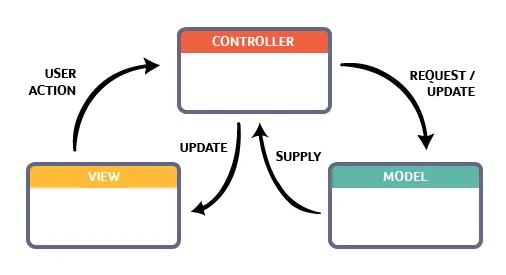
\includegraphics[width=10cm]{Images/ezgif-4-c53032b3fd.png}
%     \vspace{0.5cm}
%     \caption{MVC là gì?}
%     \label{fig:my_label}
% \end{figure}

% Mô hình MVC (MVC pattern) thường được dùng để phát triển giao diện người dùng. Nó cung cấp các thành phần cơ bản để thiết kế một chương trình cho máy tính hoặc điện thoại di động, cũng như là các ứng dụng web.

% \subsubsection{Các thành phần của MVC}
% Mô hình MVC gồm 3 loại chính là thành phần bên trong không thể thiếu khi áp dụng mô hình này:
% \begin{figure}[H]
%     \centering
%     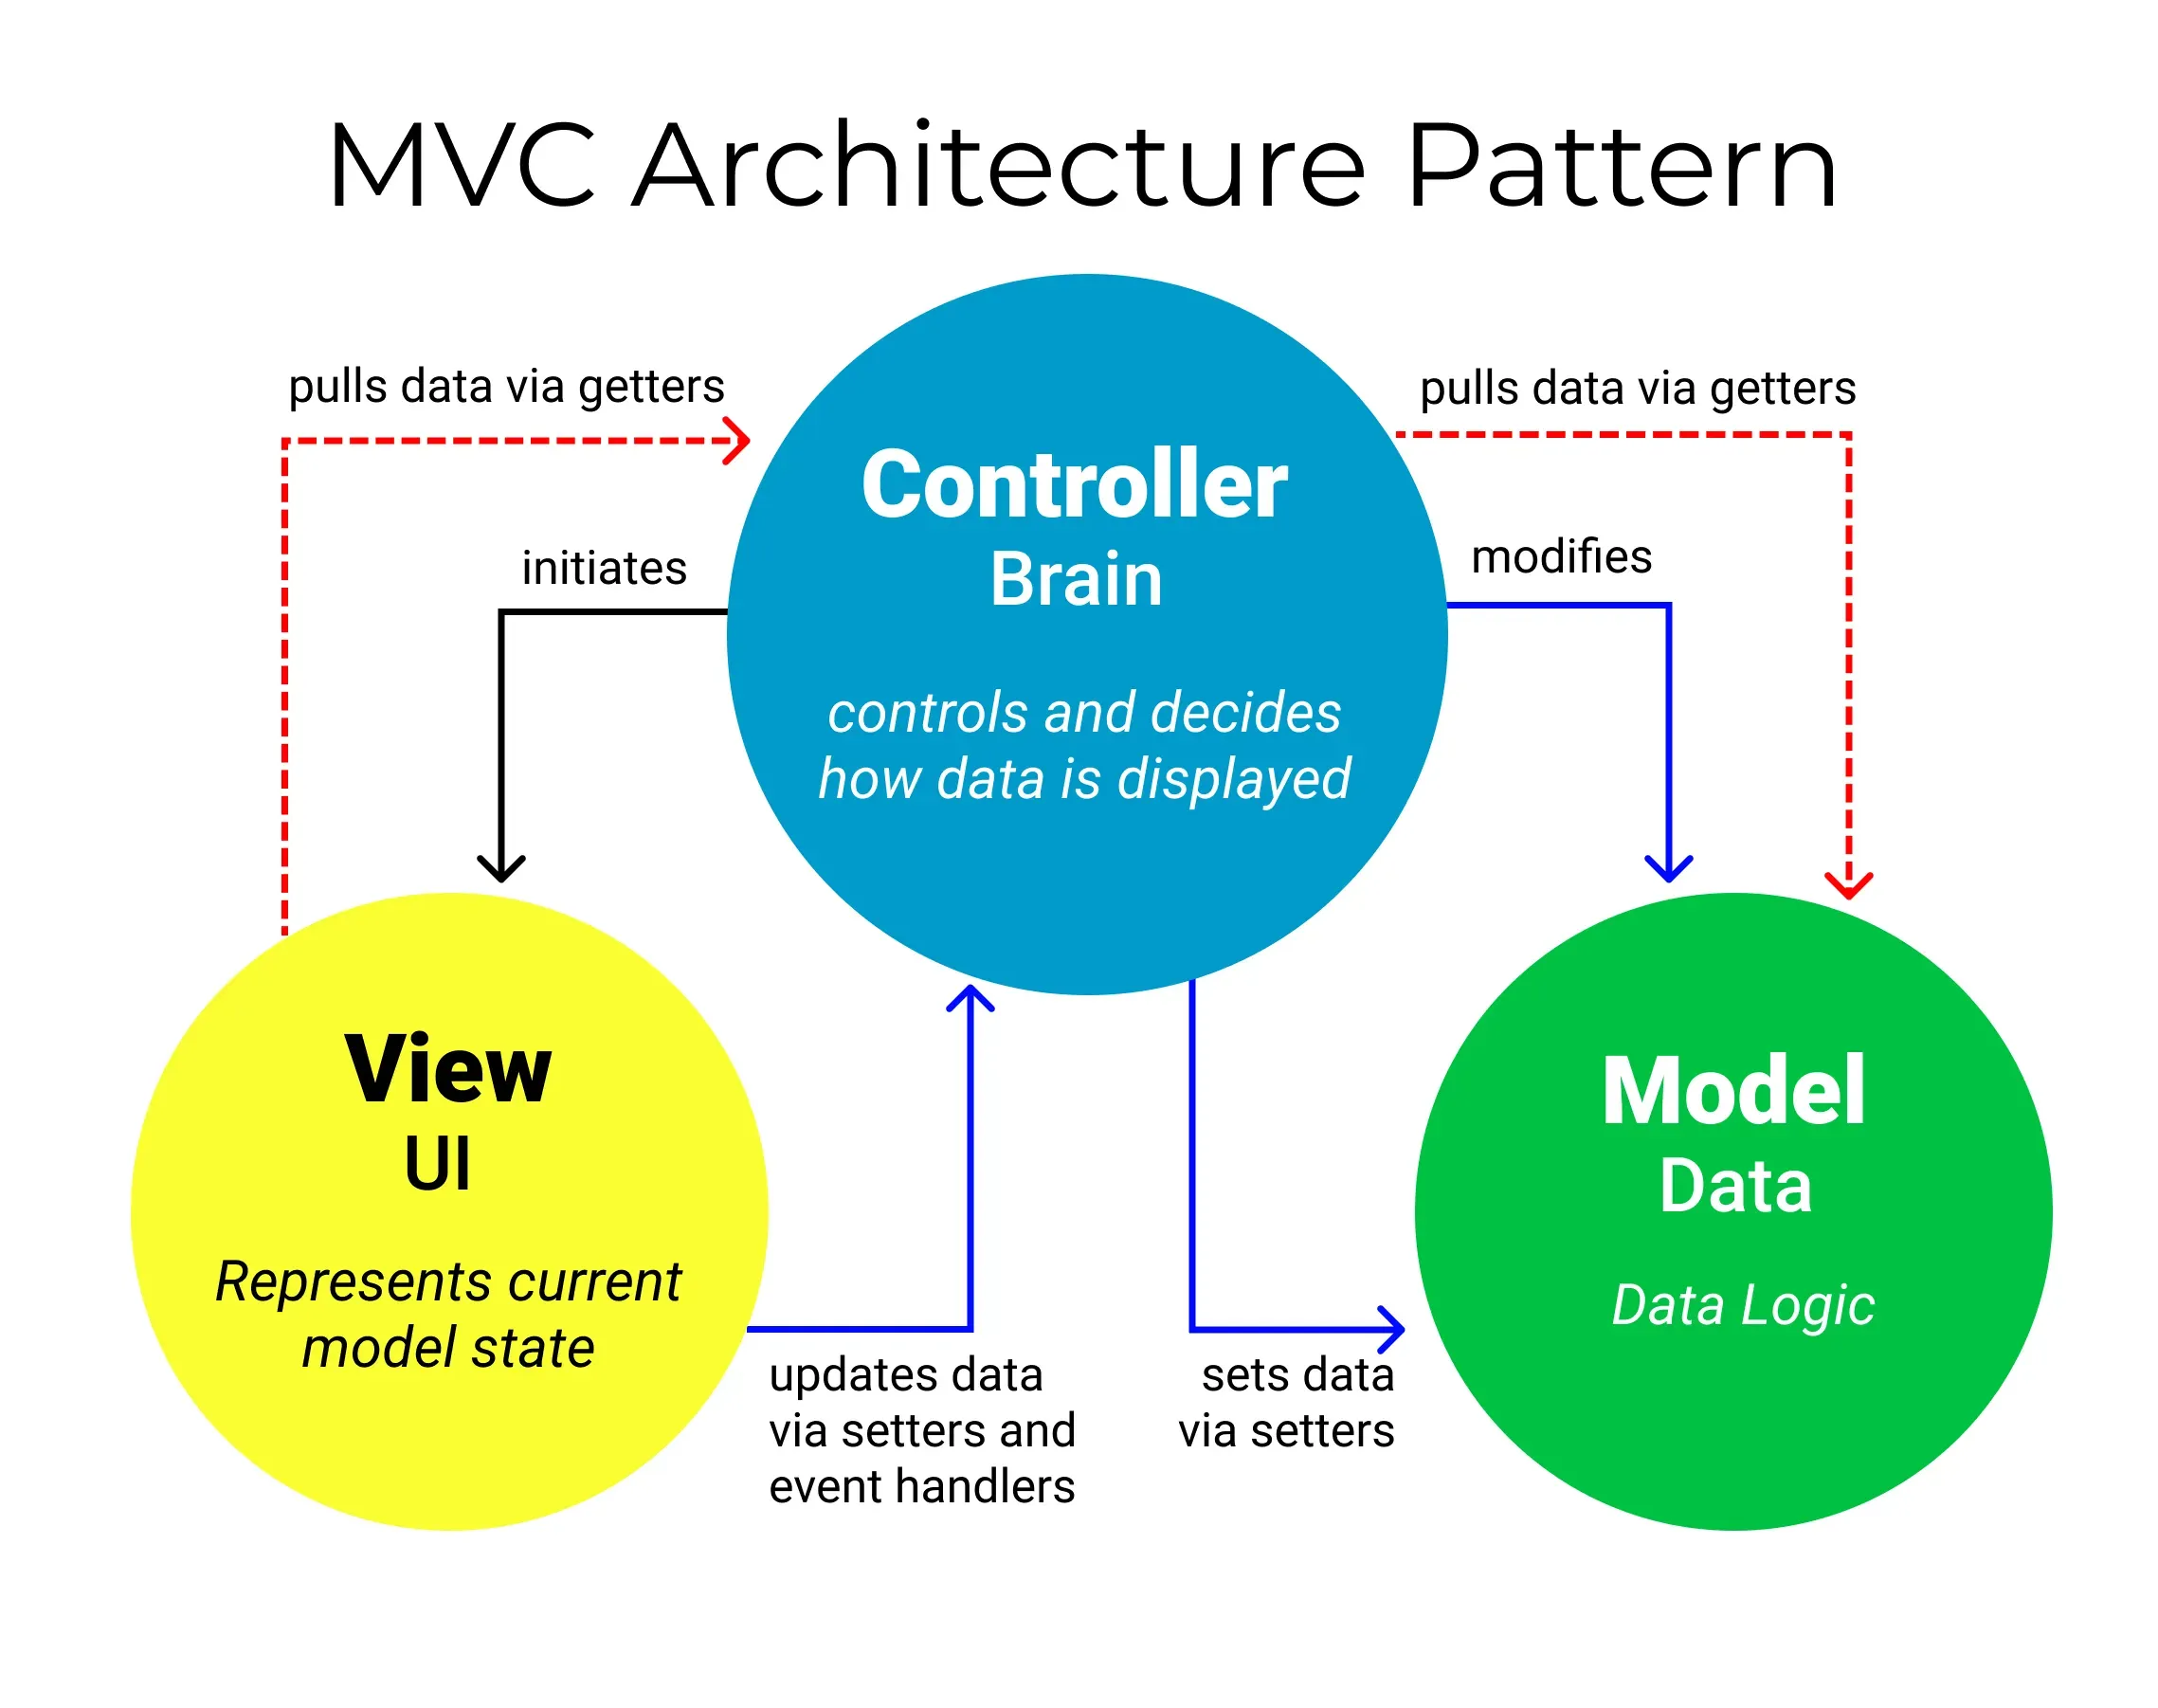
\includegraphics[width=10cm]{Images/cacthanhphanmvc.png}
%     \vspace{0.5cm}
%     \caption{Thành phần của MVC}
%     \label{fig:my_label}
% \end{figure}

% \begin{itemize}
%     \item Model: Là bộ phận có chức năng lưu trữ toàn bộ dữ liệu của ứng dụng và là cầu nối giữa 2 thành phần bên dưới là View và Controller. Một model là dữ liệu được sử dụng bởi chương trình. Đây có thể là cơ sở dữ liệu, hoặc file XML bình thường hay một đối tượng đơn giản. Chẳng hạn như biểu tượng hay là một nhân vật trong game.
%     \item View: Đây là phần giao diện (theme) dành cho người sử dụng. View là phương tiện hiển thị các đối tượng trong một ứng dụng. Chẳng hạn như hiển thị một cửa sổ, nút hay văn bản trong một cửa sổ khác. Nó bao gồm bất cứ thứ gì mà người dùng có thể nhìn thấy được.
%     \item Controller: Là bộ phận có nhiệm vụ xử lý các yêu cầu người dùng đưa đến thông qua View. Một controller bao gồm cả Model lẫn View. Nó nhận input và thực hiện các update tương ứng.
% \end{itemize}

% \subsubsection{Luồng xử lý trong MVC}
% Luồng xử lý trong của mô hình MVC, bạn có thể hình dung cụ thể và chi tiết qua từng bước dưới đây:
% \begin{itemize}
%     \item Khi một yêu cầu của từ máy khách (Client) gửi đến Server. Thì bị Controller trong MVC chặn lại để xem đó là URL request hay sự kiện.
%     \item Sau đó, Controller xử lý input của user rồi giao tiếp với Model trong MVC.
%     \item Model chuẩn bị data và gửi lại cho Controller.
%     \item Cuối cùng, khi xử lý xong yêu cầu thì Controller gửi dữ liệu trở lại View và hiển thị cho người dùng trên trình duyệt.
% \end{itemize}
% \begin{figure}[H]
%     \centering
%     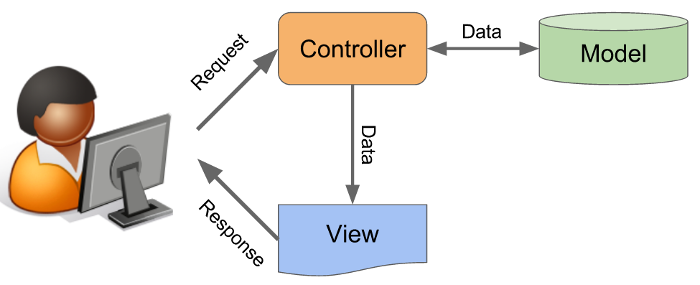
\includegraphics[width=10cm]{Images/luongmvc.png}
%     \vspace{0.5cm}
%     \caption{View và Model sẽ được xử lý bởi Controller}
%     \label{fig:my_label}
% \end{figure}

% Ở đây, View không giao tiếp trực tiếp với Model. Sự tương tác giữa View và Model sẽ chỉ được xử lý bởi Controller.
\subsubsection{Ưu và nhược điểm của MVC}
\textbf{Ưu điểm mô hình MVC}
\begin{itemize}
    \item Đầu tiên, nhắc tới ưu điểm mô hình MVC thì đó là băng thông (Bandwidth) nhẹ vì không sử dụng viewstate nên khá tiết kiệm băng thông. Việc giảm băng thông giúp website hoạt động ổn định hơn.
    \item Kiểm tra đơn giản và dễ dàng, kiểm tra lỗi phần mềm trước khi bàn giao lại cho người dùng.
    \item Một lợi thế chính của MVC là nó tách biệt các phần Model, Controller và View với nhau.
    \item Sử dụng mô hình MVC chức năng Controller có vai trò quan trọng và tối ưu trên các nền tảng ngôn ngữ khác nhau
    \item Ta có thể dễ dàng duy trì ứng dụng vì chúng được tách biệt với nhau.
    \item Có thể chia nhiều developer làm việc cùng một lúc. Công việc của các developer sẽ không ảnh hưởng đến nhau.
    \item Hỗ trợ TTD (test-driven development). Chúng ta có thể tạo một ứng dụng với unit test và viết các won test case.
    \item Phiên bản mới nhất của MVC hỗ trợ trợ thiết kế responsive website mặc định và các mẫu cho mobile. Chúng ta có thể tạo công cụ View của riêng mình với cú pháp đơn giản hơn nhiều so với công cụ truyền thống.
\end{itemize}
\textbf{Nhược điểm mô hình MVC}\\

MVC đa phần phù hợp với công ty chuyên về website hoặc các dự án lớn thì mô hình này phù hợp hơn so với với các dự án nhỏ, lẻ vì khá là cồng kềnh và mất thời gian.

\begin{itemize}
    \item Không thể Preview các trang như ASP.NET.
    \item Khó triển khai.
\end{itemize}
\subsubsection{Lý do sử dụng MVC}
\textbf{Quy trình phát triển nhanh hơn}\\

MVC hỗ trợ phát việc phát triển nhanh chóng và song song. Nếu một mô hình MVC được dùng để phát triển bất kỳ ứng dụng web cụ thể nào, một lập trình viên có thể làm việc trên View và một developer khác có thể làm việc với Controller để tạo logic nghiệp vụ cho ứng dụng web đó.\\

Do đó, ứng dụng mô hình MVC có thể được hoàn thành nhanh hơn ba lần so với các ứng dụng mô hình khác.\\

\textbf{Khả năng cung cấp nhiều chế độ view}\\

Trong mô hình MVC, bạn có thể tạo nhiều View cho chỉ một mô hình. Ngày nay, nhu cầu có thêm nhiều cách mới để truy cập ứng dụng và đang ngày càng tăng. Do đó, việc sử dụng MVC để phát triển chắc chắn là một giải pháp tuyệt vời.\\

Hơn nữa, với phương pháp này, việc nhân bản code rất hạn chế. Vì nó tách biệt dữ liệu và logic nghiệp vụ khỏi màn hình.\\

\textbf{Các sửa đổi không ảnh hưởng đến toàn bộ mô hình}\\

Đối với bất kỳ ứng dụng web nào, người dùng có xu hướng thay đổi thường xuyên. Bạn có thể quan sát thông qua những thay đổi thường xuyên về màu sắc, font chữ, bố cục màn hình. Hay là thêm hỗ trợ thiết bị mới cho điện thoại hay máy tính bảng…\\

Việc thêm một kiểu view mới trong MVC rất đơn giản. Vì phần Model không phụ thuộc vào phần View. Do đó, bất kỳ thay đổi nào trong Model sẽ không ảnh hưởng đến toàn bộ kiến trúc.\\

\textbf{MVC Model trả về dữ liệu mà không cần định dạng}\\

MVC pattern có thể trả về dữ liệu mà không cần áp dụng bất kỳ định dạng nào. Do đó, các thành phần giống nhau có thể được sử dụng với bất kỳ giao diện nào.\\

Ví dụ: tất cả loại dữ liệu đều có thể được định dạng bằng HTML. Ngoài ra, nó cũng có thể được định dạng bằng Macromedia Flash hay Dream Viewer.\\
